\chapter{Literature Review}\label{ch:lit}

% ==================================================================
\section{Introduction}\label{sec:lit-intro}
% ==================================================================
This chapter reviews the body of knowledge on which the present research builds. Because \prism{} sits at the
intersection of several disciplines, the review is deliberately broad: it spans classical traffic engineering,
adaptive and pressure-based signal control, learning-based control, roadside sensing, microscopic simulation,
drone-based data collection and computer-vision methods for vehicle detection and tracking. Each strand is
examined with a specific question in mind, namely what it contributes to, or leaves unsolved for, the control of
a single signalised junction carrying heterogeneous, non-lane-based traffic of the kind found at the Maviththara
Junction on the Piliyandala bypass.

The chapter is organised as follows. \Cref{sec:lit-fundamentals} introduces the fundamentals of signalised
intersection control and Webster's classical timing theory. \Cref{sec:lit-actuated,sec:lit-atcs} review
vehicle-actuated control and commercial adaptive systems. \Cref{sec:lit-maxpressure} examines max-pressure
control, which is the theoretical foundation of \prism{}, and \cref{sec:lit-rl} contrasts it with learning-based
approaches. \Cref{sec:lit-sensing,sec:lit-sim,sec:lit-drone,sec:lit-cv} review sensing technologies, simulation
tools, drone datasets and vision methods respectively. \Cref{sec:lit-srilanka} places the work in the Sri Lankan
context, and \cref{sec:lit-gap} distils the research gap that this dissertation addresses.

% ==================================================================
\section{Fundamentals of Signalised Intersection Control}\label{sec:lit-fundamentals}
% ==================================================================
\subsection{Terminology}
A traffic signal allocates the right of way at an intersection between conflicting streams of traffic in time
rather than in space. A \emph{movement} is a stream of vehicles travelling from one approach to one exit (for
example, a right turn from the North approach). A \emph{phase} is a set of mutually compatible movements that
receive green simultaneously, and the \emph{cycle} is one complete sequence of all phases, of length $C$
seconds. The share of the cycle given to each phase is its \emph{green split}. Between consecutive greens, an
amber (intergreen) and an all-red clearance interval separate conflicting streams; together with the start-up
delay of the first queued drivers, these produce \emph{lost time} during which the junction does not discharge
at full rate. The Traffic Signal Timing Manual \cite{koonce2008timing} and the Highway Capacity Manual (HCM)
\cite{hcm2016} codify this vocabulary and remain the principal practitioner references.

The key capacity parameter is the \emph{saturation flow} $s$, the maximum rate (vehicles or passenger car units
per hour of green per lane) at which a standing queue discharges once the initial start-up transient has
passed. If $q_i$ is the arrival flow on the critical movement of phase $i$, its \emph{flow ratio} is
$y_i = q_i/s_i$ and the intersection flow ratio is $Y=\sum_i y_i$. The capacity of a movement with effective green
$g_i$ is $s_i g_i / C$, and its \emph{degree of saturation} is $x_i = q_i C/(s_i g_i)$. The HCM measures performance
principally through \emph{control delay}, the additional travel time attributable to the signal, which is
mapped onto level-of-service categories \cite{hcm2016}.

\subsection{Webster's method}
Webster's seminal work \cite{webster1958} derived, from simulation and queueing analysis, an expression for the
average delay per vehicle on an approach,
\begin{equation}
  d = \frac{C(1-\lambda)^2}{2(1-\lambda x)} + \frac{x^2}{2q(1-x)} - 0.65\left(\frac{C}{q^2}\right)^{1/3} x^{(2+5\lambda)},
  \label{eq:webster-delay}
\end{equation}
where $\lambda = g/C$ is the proportion of the cycle that is effectively green. The first term is the uniform
delay of regular arrivals, the second a random (overflow) term derived from queueing theory, and the third an
empirical correction. Minimising total delay with respect to $C$ yields the well-known optimal cycle length
\begin{equation}
  C_0 = \frac{1.5L + 5}{1 - Y},
  \label{eq:webster-c0}
\end{equation}
where $L$ is the total lost time per cycle. Effective green is then shared in proportion to the critical flow
ratios, $g_i = (C_0 - L)\,y_i/Y$ \cite{webster1958,koonce2008timing}. \Cref{fig:webster-c0} illustrates the
characteristic behaviour of \cref{eq:webster-c0}: as $Y$ approaches unity the optimal cycle grows without bound,
which is why fixed-time plans become fragile precisely at the high demand levels observed during the morning peak
at Maviththara. Webster's method is used in this research to construct the ``best fixed-time'' baseline (B3).

\begin{figure}[H]
  \centering
  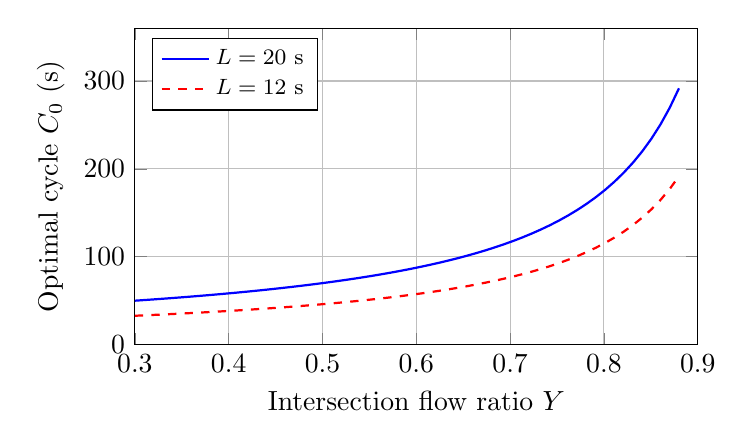
\begin{tikzpicture}
    \begin{axis}[width=0.72\textwidth,height=5.6cm,xlabel={Intersection flow ratio $Y$},
        ylabel={Optimal cycle $C_0$ (s)},xmin=0.3,xmax=0.9,ymin=0,ymax=360,grid=major,
        legend pos=north west,legend style={font=\footnotesize}]
      \addplot[thick,blue,domain=0.3:0.88,samples=60]{(1.5*20+5)/(1-x)};
      \addlegendentry{$L=20$ s}
      \addplot[thick,dashed,red,domain=0.3:0.88,samples=60]{(1.5*12+5)/(1-x)};
      \addlegendentry{$L=12$ s}
    \end{axis}
  \end{tikzpicture}
  \caption{Webster's optimal cycle length (\cref{eq:webster-c0}) as a function of the intersection flow ratio
  for two values of total lost time. $L=20$ s corresponds to four phases with 5 s interphase each.}
  \label{fig:webster-c0}
\end{figure}

\subsection{Traffic flow theory}
At a more fundamental level, queue formation and dissipation at a signal are described by the kinematic wave
theory of Lighthill and Whitham \cite{lighthill1955}, in which traffic is treated as a compressible fluid and
changes in density propagate as waves. At the onset of red a shock wave propagates upstream as arriving vehicles
join the queue; at the onset of green a discharge wave travels back through the queue at a speed governed by the
jam density and the saturation flow. This macroscopic picture underlies both the queue-clearance logic of
\prism{}'s green-time estimate and the interpretation of queue lengths in the simulation results. Treiber and
Kesting \cite{treiber2013} provide a modern synthesis that connects these macroscopic models to the
microscopic car-following models used in simulators.

\subsection{Passenger car units}
All of the above formulations assume a homogeneous stream of ``standard'' vehicles. Where traffic is mixed, the
common remedy is to express flows in \emph{passenger car units} (PCU), weighting each vehicle by its equivalent
impact on capacity relative to a passenger car. The Indian Roads Congress guideline IRC:106 \cite{irc106}
tabulates PCU factors for urban roads in mixed traffic, including two-wheelers, auto-rickshaws (three-wheelers),
buses and trucks, and is widely referenced across South Asia. The PCU concept is central to this research:
\prism{} measures queues and arrivals in PCU rather than in vehicle counts, so that a queue of ten motorcycles is
not treated as equivalent to a queue of ten buses.

% ==================================================================
\section{Fixed-Time and Vehicle-Actuated Control}\label{sec:lit-actuated}
% ==================================================================
\emph{Fixed-time} (pre-timed) control repeats a predetermined cycle, split and phase sequence, possibly with
different plans for different times of day. Its advantages are simplicity, predictability, zero dependence on
detectors and ease of coordination along arterials \cite{koonce2008timing}. Its fundamental weakness is that the
plan is optimised for an assumed demand; when actual arrivals deviate, green is wasted on empty approaches while
queues grow elsewhere. The Maviththara Junction currently operates in this mode.

\emph{Vehicle-actuated} control introduces local feedback from detectors, usually inductive loops placed
upstream of the stop line. Each phase is bounded by a \emph{minimum green}, which guarantees that the standing
queue between the detector and stop line can start up safely, and a \emph{maximum green}, which caps the waiting
time of conflicting movements. Between these bounds the green is extended by a \emph{passage time} (unit
extension) each time a vehicle is detected; when the time since the last detection exceeds the allowed gap, the
phase ``gaps out'' and the controller advances to the next phase with demand \cite{koonce2008timing}. SUMO
implements this logic in its built-in \texttt{actuated} traffic-light type, which extends phases while vehicles
are detected within a configurable maximum gap, subject to \texttt{minDur} and \texttt{maxDur}
\cite{sumo_actuated}; this implementation forms baseline B2 of the evaluation.

Actuated control is myopic: it reacts only to the phase currently served and ignores the size of competing queues.
Under heavy demand every phase tends to run to maximum green, so the controller degenerates into fixed-time
operation at the maximum settings. Moreover, a detector pulse does not distinguish a motorcycle from a bus, and
motorcycles filtering laterally can be missed entirely by lane-based loops. Both limitations are acute in
heterogeneous traffic.

% ==================================================================
\section{Adaptive Traffic Signal Control Systems}\label{sec:lit-atcs}
% ==================================================================
Adaptive traffic control systems (ATCS) continuously adjust timings in response to measured demand. Papageorgiou
\emph{et al.} \cite{papageorgiou2003review} provide a comprehensive review of road traffic control strategies,
and Stevanovic's NCHRP Synthesis \cite{stevanovic2010nchrp} surveys the state of practice of ATCS deployment,
including agency experience of their benefits, costs and operational challenges. The principal systems are
summarised below.

\textbf{SCOOT} (Split, Cycle and Offset Optimisation Technique), developed by the UK Transport and Road Research
Laboratory \cite{hunt1981scoot}, uses detectors located upstream of the stop line to build cyclic flow profiles,
which feed an on-line model of queues. It makes frequent, small incremental adjustments to splits, offsets and
cycle times to reduce a performance index combining delay and stops across a network.

\textbf{SCATS} (Sydney Coordinated Adaptive Traffic System) \cite{sims1980scats} adopts a hierarchical
architecture in which regional computers adjust cycle length, splits and offsets based on a measure of the
degree of saturation computed from stop-line detectors, and select among stored plans, while local controllers
retain tactical, actuated-style control.

\textbf{OPAC} (Optimisation Policies for Adaptive Control) \cite{gartner1983opac} formulates signal timing as an
optimisation over a rolling horizon, using detector data and short-term arrival predictions to choose switching
times that minimise delay without being constrained to a fixed cycle. \textbf{RHODES} \cite{mirchandani2001rhodes}
similarly uses a hierarchical, prediction-based architecture combining network flow, platoon prediction and
intersection-level phase optimisation. \textbf{SURTRAC} \cite{xie2012surtrac} treats each intersection as a
scheduling problem over clusters of approaching vehicles, solved in real time and coordinated with neighbours
through the exchange of predicted outflows, achieving decentralised network coordination.

These systems have demonstrated benefits in many cities, yet their transferability to suburban junctions in
developing countries is limited for three reasons. First, they are proprietary or require significant licensing,
central infrastructure and specialist staff; the NCHRP synthesis notes that cost and detector maintenance are
recurrent concerns among agencies \cite{stevanovic2010nchrp}. Second, they depend on dense inductive loop
detection whose installation requires cutting the carriageway and whose failure degrades performance. Third,
their traffic models assume lane-disciplined streams of predominantly four-wheeled vehicles: a loop occupancy
or count does not reflect the true PCU load where motorcycles and three-wheelers travel side by side, overtake
within a lane and accumulate ahead of the stop line. These observations motivate a controller that is both
algorithmically simple and fed by a sensor that perceives every road user regardless of lane position.

% ==================================================================
\section{Max-Pressure and Back-Pressure Control}\label{sec:lit-maxpressure}
% ==================================================================
\subsection{Origins and theory}
The concept of back-pressure scheduling originates in communication networks. In their
work on multihop radio networks, Tassiulas and Ephremides \cite{tassiulas1992} studied constrained queueing networks, in which only certain sets of servers can be active simultaneously, and
showed that a policy which activates the feasible set with the maximum weighted queue differential
is optimal in throughput: it stabilises the network for every arrival rate vector that any policy could stabilise.
A signalised road network has precisely this structure, with phases playing the role of feasible activation sets.

Varaiya \cite{varaiya2013maxpressure} transferred this idea to traffic signals as \emph{max-pressure} control.
Let $x_{l}(t)$ be the number of vehicles queued on link $l$, $r(l,m)$ the turning ratio from link $l$ to link $m$,
and $c(l,m)$ the saturation flow of movement $(l,m)$. The \emph{weight} of a movement is
\begin{equation}
  w_{l,m}(t) = x_l(t) - \sum_{p} r(m,p)\, x_m(t),
  \label{eq:mp-weight}
\end{equation}
that is, the upstream queue minus the turning-ratio-weighted downstream queue. The \emph{pressure} of a phase
(or stage) $j$ is
\begin{equation}
  P_j(t) = \sum_{(l,m)\in j} w_{l,m}(t)\, c(l,m),
  \label{eq:mp-pressure}
\end{equation}
and at each decision instant the controller activates
\begin{equation}
  j^\ast(t) = \arg\max_{j} P_j(t).
  \label{eq:mp-argmax}
\end{equation}
Varaiya proved, under a store-and-forward queueing model, that this policy stabilises queues whenever demand lies
within the capacity region, without requiring any knowledge of the demand itself. The controller is fully
decentralised: each intersection uses only the queues on its own incoming and outgoing links, so the
computation scales trivially to large networks.

\subsection{Extensions}
Kouvelas \emph{et al.} \cite{kouvelas2014maxpressure} examined max-pressure control for signalised arterial
networks in simulation and investigated practical variants, including the allocation of green within a cycle in
proportion to pressure, demonstrating its potential to stabilise queues in realistic settings. Wongpiromsarn
\emph{et al.} \cite{wongpiromsarn2012distributed} proposed a distributed back-pressure signal controller and
established its maximum network throughput property. Gregoire \emph{et al.} \cite{gregoire2015capacity} observed
that the original formulation implicitly assumes unbounded link capacity, and introduced a capacity-aware
variant that normalises queues by link capacity so that pressure correctly accounts for downstream links that
are close to full, thereby mitigating spillback.

\subsection{Limitations relevant to this research}
Despite its theoretical appeal, the classical formulation rests on assumptions that do not hold at a junction
such as Maviththara:
\begin{enumerate}[leftmargin=*,itemsep=2pt]
  \item \textbf{Vehicle counts.} Queues $x_l$ are counted in vehicles, implicitly assuming homogeneous vehicles.
        In Sri Lankan traffic, a bus occupies several times the road space and discharge time of a motorcycle.
  \item \textbf{Fixed time slots.} The theory is developed for decisions at fixed slot boundaries, with phase
        changes incurring no loss. In practice every switch costs amber and all-red time, so naive per-second
        switching wastes capacity, while long slots ignore actual queue clearance.
  \item \textbf{Full observability.} Exact queue lengths on all incoming and outgoing links are assumed to be
        known. Real sensors have limited range, noise, missed detections and occlusion.
  \item \textbf{No fairness guarantee.} Stability is a long-run property; an approach with persistently low
        pressure can, in the short term, wait for an unacceptably long time.
\end{enumerate}
\prism{} directly addresses each of these: pressure is computed in PCU from LiDAR size classes; green duration
is variable, bounded by minimum and maximum greens and informed by a queue-clearance estimate with hysteresis;
the state is estimated from a noisy virtual LiDAR with a perception tracker; and an urgency multiplier together
with a starvation cap provides an explicit fairness guarantee (see \cref{sec:prism}).

% ==================================================================
\section{Learning-Based Signal Control}\label{sec:lit-rl}
% ==================================================================
Reinforcement learning (RL) frames signal control as a sequential decision problem in which an agent observes the
traffic state, selects a phase and receives a reward such as negative delay. Abdulhai \emph{et al.}
\cite{abdulhai2003rl} applied Q-learning to an isolated intersection and argued that RL offers ``true''
adaptivity because it does not require a pre-specified traffic model. Arel \emph{et al.} \cite{arel2010rl}
extended the approach to a multi-agent setting with function approximation for network control. With the advent
of deep learning, Genders and Razavi \cite{genders2016drl} trained a deep RL agent on a high-resolution
representation of vehicle positions and speeds, and Wei \emph{et al.} \cite{wei2018intellilight} proposed
IntelliLight, which was evaluated with large-scale real-world traffic data. Wei \emph{et al.} \cite{wei2019survey}
survey the field and compare transportation-engineering and RL methods, notably including max-pressure as a
strong classical baseline.

Learning-based methods have achieved impressive simulation results, but several concerns limit their adoption by
traffic authorities, especially in resource-constrained settings:
\begin{itemize}[leftmargin=*,itemsep=2pt]
  \item \textbf{Opacity.} A neural policy cannot easily be explained to the engineers who must approve it, nor
        audited after an incident.
  \item \textbf{Data and compute demands.} Training typically requires very large numbers of simulated episodes
        and GPU resources, and must be repeated when the junction or demand changes.
  \item \textbf{Sim-to-real gap.} A policy optimised against a simulator may exploit modelling artefacts and
        behave unpredictably under real sensor noise or unseen conditions.
  \item \textbf{Safety certification.} Without formal guarantees, constraints such as minimum green and maximum
        red must be enforced by external wrappers.
\end{itemize}
By contrast, max-pressure control is analytically grounded, has provable stability properties and requires no
training. This research therefore deliberately confines artificial intelligence to the \emph{offline} data
extraction pipeline (vehicle detection), while the on-line controller remains a transparent mathematical rule
whose every decision can be traced to measured PCU quantities.

% ==================================================================
\section{Traffic Sensing Technologies}\label{sec:lit-sensing}
% ==================================================================
Any adaptive controller is only as good as its measurement of traffic state. \emph{Inductive loop detectors}
are the incumbent technology for SCOOT, SCATS and actuated control; they are accurate for presence and counts of
lane-following vehicles, but are intrusive to install and maintain, measure only at a point, and frequently
fail to register small vehicles travelling off the lane centre. \emph{Video cameras} combined with computer
vision provide rich, wide-area information and can classify vehicles, but performance degrades at night, in
heavy rain and under glare, and they raise privacy concerns because faces and number plates may be captured.
\emph{Radar} is robust to weather and lighting and measures speed directly, but offers limited spatial
resolution for classifying closely spaced small vehicles.

\emph{LiDAR} (light detection and ranging) measures the three-dimensional geometry of the scene with an active
laser and is therefore largely independent of ambient lighting. Zhao \emph{et al.} \cite{zhao2019lidar} developed
a processing pipeline for detecting, classifying and tracking pedestrians and vehicles from roadside LiDAR, and
Lv \emph{et al.} \cite{lv2019lidar} demonstrated LiDAR-enhanced connected infrastructure that extracts and
broadcasts high-resolution traffic information. Commercial multi-channel sensors such as the Ouster OS1 family
\cite{ouster_os1} offer a 360\textdegree{} field of view with ranges suitable for covering an entire junction from a
single pole. Finally, \emph{connected vehicles} can report their own positions and speeds directly; Goodall
\emph{et al.} \cite{goodall2013cv} showed that signal control using connected-vehicle data can reduce delay, but
benefits depend on market penetration, which is negligible in Sri Lanka at present. \Cref{tab:lit-sensors}
compares these options qualitatively.

\begin{table}[H]
\centering
\caption{Qualitative comparison of traffic sensing technologies for junction control (synthesised from
\cite{koonce2008timing,zhao2019lidar,lv2019lidar,goodall2013cv,stevanovic2010nchrp}).}
\label{tab:lit-sensors}
\small
\footnotesize\setlength{\tabcolsep}{3pt}
\begin{tabularx}{\textwidth}{>{\raggedright\arraybackslash}p{2.1cm} *{5}{>{\raggedright\arraybackslash}X}}
\toprule
Criterion & Inductive loop & Video camera & Radar & Roadside LiDAR & Connected vehicles \\
\midrule
Capital cost & Low per loop, high installation & Low--medium & Medium & Medium--high (falling) & Low (if fleet equipped) \\
Coverage & Point & Wide area & Wide area & 360\textdegree{}, whole junction & Equipped vehicles only \\
Night / weather & Robust & Poor at night, rain & Robust & Robust at night; moderate in heavy rain & Robust \\
Privacy & High & Low (identifiable) & High & High (no imagery) & Medium \\
Vehicle size / class & Weak & Good & Weak & Good (3-D extent) & Self-reported \\
Lane-less, mixed traffic & Poor & Good & Moderate & Good & Penetration-limited \\
Installation impact & Road cutting & Pole mount & Pole mount & Pole mount & None \\
\bottomrule
\end{tabularx}
\end{table}

For the problem at hand LiDAR offers a compelling combination. It operates equally well by day and night, which
matters because congestion on the Piliyandala bypass routinely persists after dark during the evening peak; it records
only point clouds, so individuals cannot be identified; and its three-dimensional geometry yields vehicle length
and height, from which a size class and hence a PCU weight can be inferred without a learned classifier. Its
principal disadvantage, cost, has declined markedly, and a single pole-mounted unit can replace many loops. These
arguments underpin the design of the Virtual LiDAR Sensor (\vls{}) described in \cref{sec:vls}.

% ==================================================================
\section{Simulation of Traffic and Sensors}\label{sec:lit-sim}
% ==================================================================
Microscopic simulation is the standard means of evaluating signal-control strategies before field deployment.
SUMO (Simulation of Urban MObility) \cite{lopez2018sumo} is an open-source, multi-modal microscopic simulator that
supports large networks, multiple vehicle classes, detailed output of trip, queue and emission statistics, and
on-line control through the Traffic Control Interface (TraCI) \cite{wegener2008traci}, which allows an external
program to read the simulation state and set signal states at every step. This makes SUMO particularly well
suited to testing a custom controller.

SUMO's default car-following model is that of Krau{\ss} \cite{krauss1998}, a stochastic, collision-free model in
which each driver adopts a ``safe speed'' and randomly decelerates by an amount governed by an imperfection
parameter $\sigma$. Lane changing follows Erdmann's model \cite{erdmann2015lanechange}, which considers strategic,
cooperative, speed-gain and keep-right motivations. Crucially for heterogeneous traffic, SUMO also provides a
\emph{sublane model} \cite{sumo_sublane} that discretises each lane into narrow lateral strips, allowing several
narrow vehicles to travel side by side and motorcycles to filter between cars towards the stop line. This
capability is essential for reproducing Sri Lankan queue formation and is adopted in this work.

For sensor simulation, CARLA \cite{dosovitskiy2017carla} offers physically based camera and LiDAR rendering
within an urban driving environment. However, it is oriented towards autonomous-vehicle research and is
computationally heavy for hour-long, multi-seed traffic experiments. This research instead implements a
lightweight analytical LiDAR model over SUMO's vehicle state, capturing range limits, noise, dropout and
occlusion at a fraction of the cost.

A simulation is credible only if calibrated against observation. The FHWA Traffic Analysis Toolbox
\cite{dowling2004toolbox} provides widely adopted guidance, including the GEH statistic,
\begin{equation}
  \mathrm{GEH} = \sqrt{\frac{2(M-C)^2}{M+C}},
  \label{eq:geh}
\end{equation}
where $M$ is the modelled and $C$ the counted hourly flow, with the criterion that GEH should be below 5 for at
least 85\% of cases. Mathew and Radhakrishnan \cite{mathew2010calibration} addressed calibration of
microsimulation models specifically for non-lane-based heterogeneous traffic at signalised intersections in India,
demonstrating that default parameters are inadequate and that systematic calibration of driver-behaviour
parameters is required for such conditions. Treiber and Kesting \cite{treiber2013} further discuss
parameter identification for car-following models.

% ==================================================================
\section{Drone-Based Traffic Data Collection}\label{sec:lit-drone}
% ==================================================================
Unmanned aerial vehicles (drones) have emerged as a powerful tool for collecting naturalistic trajectory data.
A hovering drone with a nadir camera observes an entire junction without occlusion by large vehicles and without
roadside installation. The highD dataset \cite{krajewski2018highd} provides drone-recorded vehicle trajectories
from German highways for the validation of automated driving systems, demonstrating that high positional
accuracy is achievable from aerial video. The pNEUMA experiment \cite{barmpounakis2020pneuma} deployed a swarm of
drones over the congested centre of Athens and released a large-scale urban trajectory dataset, showing the
value of drone data for studying urban traffic, including mixed traffic with many powered two-wheelers.
VisDrone \cite{zhu2022visdrone} is a large benchmark for object detection and tracking from drone imagery
collected across several Chinese cities; its categories include motorcycles, tricycles and awning-tricycles,
the last of which closely resemble Sri Lankan three-wheelers. These works establish the feasibility of drone
footage as ground truth; the present research adapts the approach to a single Sri Lankan junction to extract
demand, turning ratios, saturation flow and waiting times for calibration.

% ==================================================================
\section{Object Detection and Tracking of Vehicles}\label{sec:lit-cv}
% ==================================================================
\subsection{Detectors}
Modern object detectors fall into two families. \emph{Two-stage} detectors, exemplified by Faster R-CNN
\cite{ren2015faster}, first propose candidate regions with a region proposal network and then classify and refine
them, generally achieving high accuracy at a higher computational cost. \emph{Single-stage} detectors, beginning
with YOLO \cite{redmon2016yolo}, predict boxes and classes in one pass and are designed for real-time operation.
The YOLO family has evolved considerably; YOLOv7 \cite{wang2023yolov7} introduced trainable ``bag-of-freebies''
techniques, and Ultralytics YOLOv8 \cite{jocher2023yolov8} adopted an anchor-free head and an integrated training
and deployment toolchain. Transformer-based detectors culminated in RT-DETR \cite{zhao2024rtdetr}, which removes
the need for non-maximum suppression and reports competitive real-time accuracy. Most detectors are pre-trained on
COCO \cite{lin2014coco}, whose everyday-perspective imagery differs greatly from nadir drone views.

Vehicles in 4K aerial footage captured from a high hovering altitude are small; a motorcycle may span only some twenty pixels.
Down-sampling the frame to the network input size destroys such objects. Slicing Aided Hyper Inference (SAHI)
\cite{akyon2022sahi} addresses this by running the detector on overlapping tiles and merging the results, and by
fine-tuning on sliced images, giving significant gains for small objects on aerial benchmarks.

\subsection{Multi-object trackers}
Tracking-by-detection links per-frame detections into trajectories. SORT \cite{bewley2016sort} combines a Kalman
filter motion model with Hungarian assignment on bounding-box overlap and is extremely fast. DeepSORT
\cite{wojke2017deepsort} adds a learned appearance descriptor to reduce identity switches during occlusion, at the
cost of an additional re-identification network. ByteTrack \cite{zhang2022bytetrack} observes that discarding
low-confidence detections loses partially occluded objects, and associates \emph{every} detection box in two
stages: first high-confidence boxes, then low-confidence boxes against remaining tracks. Tracking quality is
measured by the CLEAR MOT metrics \cite{bernardin2008clearmot}, notably multiple object tracking accuracy (MOTA),
which aggregates misses, false positives and identity switches, and by the identity-based IDF1 score
\cite{ristani2016idf1}, which rewards trackers that preserve consistent identities over time.

\subsection{Selection}
\Cref{tab:lit-detectors} summarises the candidates. YOLOv8 was selected because it offers a strong balance of
accuracy and speed, mature tooling for fine-tuning and export, straightforward integration with SAHI, and
publicly available VisDrone-pretrained weights. ByteTrack was selected because, in a top-down view, vehicles
of the same class look nearly identical, so appearance embeddings add little discriminative power, whereas
recovering low-confidence boxes of partially occluded motorcycles is valuable.

\begin{table}[H]
\centering
\caption{Comparison of candidate detectors and trackers for drone-based vehicle extraction (qualitative, from the
cited literature).}
\label{tab:lit-detectors}
\small
\begin{tabularx}{\textwidth}{l l >{\raggedright\arraybackslash}X >{\raggedright\arraybackslash}X}
\toprule
Method & Type & Strengths & Weaknesses for this task \\
\midrule
Faster R-CNN \cite{ren2015faster} & Two-stage detector & High accuracy, well understood & Slow for long 4K videos; heavier fine-tuning \\
YOLOv7 \cite{wang2023yolov7} & Single-stage detector & Fast, accurate & Less integrated tooling for tiling and export \\
YOLOv8 \cite{jocher2023yolov8} & Single-stage, anchor-free & Fast, mature toolchain, VisDrone weights, SAHI support & Small objects need tiling \\
RT-DETR \cite{zhao2024rtdetr} & Transformer detector & NMS-free, competitive accuracy & Higher training cost; less mature ecosystem \\
\midrule
SORT \cite{bewley2016sort} & IoU + Kalman & Very fast, simple & Drops low-score boxes; identity switches \\
DeepSORT \cite{wojke2017deepsort} & + appearance & Fewer switches in pedestrian scenes & Re-ID net of little use for top-down vehicles \\
ByteTrack \cite{zhang2022bytetrack} & Two-stage association & Retains occluded, low-score objects; no Re-ID & Sensitive to detection thresholds \\
\bottomrule
\end{tabularx}
\end{table}

% ==================================================================
\section{The Sri Lankan and Developing-Country Context}\label{sec:lit-srilanka}
% ==================================================================
Traffic in Sri Lanka, as in much of South and South-East Asia, is \emph{heterogeneous} and \emph{non-lane-based}.
Department of Motor Traffic registration statistics \cite{dmt_stats} show that motorcycles form the largest
category of the vehicle fleet, with three-wheelers also forming a substantial share. These vehicles weave
between cars, occupy gaps across lane boundaries and accumulate ahead of larger vehicles at the stop line, so
that lane-based counts and vehicle-based queue measures misrepresent the true load on an approach. The JICA
Comprehensive Urban Transport study for the Colombo Metropolitan Region (CoMTrans) \cite{jica2014comtrans}
documented growing congestion in the region and highlighted the need for improved traffic management alongside
investment in public transport.

At signalised junctions in suburban Colombo, control is typically fixed-time. When queues become severe, traffic
police frequently switch the signals off and direct traffic manually. Manual control can respond to visible
queues but is labour-intensive, inconsistent between officers, and exposes personnel to fumes and danger. To the
best of the author's knowledge, no adaptive system has been deployed at suburban junctions such as Maviththara,
and published studies of heterogeneous traffic have concentrated on capacity estimation and simulation
calibration \cite{irc106,mathew2010calibration} rather than on low-cost adaptive control.

% ==================================================================
\section{Research Gap}\label{sec:lit-gap}
% ==================================================================
The review reveals the following gaps:
\begin{itemize}[leftmargin=*,itemsep=2pt]
  \item Commercial adaptive systems \cite{hunt1981scoot,sims1980scats,gartner1983opac,mirchandani2001rhodes,xie2012surtrac}
        are costly, loop-dependent and modelled on lane-disciplined, largely four-wheeled traffic.
  \item Max-pressure control \cite{varaiya2013maxpressure,kouvelas2014maxpressure,gregoire2015capacity} offers a
        simple, decentralised and provably stabilising rule, but is formulated in vehicle counts with full
        observability and has not been adapted to PCU-weighted heterogeneous traffic or to realistic sensor error.
  \item Learning-based controllers \cite{genders2016drl,wei2018intellilight} are opaque, data-hungry and hard to
        certify, which is a barrier to adoption by road authorities.
  \item Roadside LiDAR has been shown to detect and track road users \cite{zhao2019lidar,lv2019lidar}, but its
        use as the sole input to a signal controller, with explicit modelling of its errors, is little explored.
  \item Drone trajectory datasets \cite{krajewski2018highd,barmpounakis2020pneuma} have not been used to calibrate
        a simulation of a Sri Lankan junction for the evaluation of adaptive control.
  \item No published work combines these elements for the Sri Lankan context.
\end{itemize}
\Cref{tab:lit-gap} maps representative works against the features targeted by this research.

\begin{table}[H]
\centering
\caption{Feature comparison of representative works and this research
(\checkmark{} = addressed, $\sim$ = partially, $\times$ = not addressed).}
\label{tab:lit-gap}
\small
\begin{tabularx}{\textwidth}{X c c c c c c}
\toprule
Work & \shortstack{Hetero.\\PCU} & \shortstack{LiDAR\\sensing} & \shortstack{No-ML\\control} & \shortstack{Low\\cost} & \shortstack{Drone\\calib.} & \shortstack{Sri Lankan\\context} \\
\midrule
SCOOT / SCATS \cite{hunt1981scoot,sims1980scats} & $\times$ & $\times$ & \checkmark & $\times$ & $\times$ & $\times$ \\
OPAC / RHODES \cite{gartner1983opac,mirchandani2001rhodes} & $\times$ & $\times$ & \checkmark & $\times$ & $\times$ & $\times$ \\
SURTRAC \cite{xie2012surtrac} & $\times$ & $\times$ & \checkmark & $\sim$ & $\times$ & $\times$ \\
Max-pressure \cite{varaiya2013maxpressure,kouvelas2014maxpressure} & $\times$ & $\times$ & \checkmark & \checkmark & $\times$ & $\times$ \\
Capacity-aware BP \cite{gregoire2015capacity} & $\times$ & $\times$ & \checkmark & \checkmark & $\times$ & $\times$ \\
Deep RL \cite{genders2016drl,wei2018intellilight} & $\times$ & $\times$ & $\times$ & $\sim$ & $\times$ & $\times$ \\
Connected vehicles \cite{goodall2013cv} & $\times$ & $\times$ & \checkmark & $\sim$ & $\times$ & $\times$ \\
Roadside LiDAR \cite{zhao2019lidar,lv2019lidar} & $\sim$ & \checkmark & -- & $\sim$ & $\times$ & $\times$ \\
Heterogeneous calibration \cite{mathew2010calibration} & \checkmark & $\times$ & -- & -- & $\times$ & $\times$ \\
Drone datasets \cite{barmpounakis2020pneuma,zhu2022visdrone} & $\sim$ & $\times$ & -- & -- & \checkmark & $\times$ \\
\midrule
\textbf{This work (\prism{})} & \checkmark & \checkmark & \checkmark & \checkmark & \checkmark & \checkmark \\
\bottomrule
\end{tabularx}
\end{table}

% ==================================================================
\section{Chapter Summary}\label{sec:lit-summary}
% ==================================================================
This chapter has traced the development of signal control from Webster's fixed-time theory, through actuated and
adaptive systems, to max-pressure control and reinforcement learning. Max-pressure emerged as an attractive
foundation because it is decentralised, analytically grounded and requires only local measurements, but its
assumptions of homogeneous vehicles, fixed slots, perfect observation and implicit fairness must be relaxed for
heterogeneous traffic. Roadside LiDAR was identified as a sensor that suits lane-less mixed traffic, operates at
night and preserves privacy; SUMO with its sublane model, calibrated from drone footage processed with YOLOv8 and
ByteTrack, was identified as an appropriate evaluation environment. The following chapter (\cref{ch:method})
describes the methodology by which these elements were combined into \prism{}.
